\documentclass[]{jarticle}          % 一段組
%\documentclass[twocolumn]{jarticle} % 二段組

\textwidth 180mm
\textheight 255mm
\oddsidemargin -12mm
\topmargin -15mm
\columnsep 10mm

%\vspace{0.5cm} % 一段組の場合はコメントアウトした方が体裁がよいx
%] % 一段組の場合はコメントアウトする

\usepackage{styles/labheadings}
\usepackage[dvipdfmx]{graphicx,color}
\usepackage{amsmath,amssymb}
\usepackage{url}
% 追加
\usepackage[hang,small,bf]{caption}
\usepackage[subrefformat=parens]{subcaption}
\usepackage{float}
\captionsetup{compatibility=false}

\input{numerical_definition.tex}
% report.texと同じディレクトリにnumerical_definition.texを入れておけば上の書き方でもいいはずです

\usepackage[
  dvipdfm,
  bookmarks=true,
  bookmarksnumbered=true,
  colorlinks=true]{hyperref}
\AtBeginDvi{\special{pdf:tounicode EUC-UCS2}}

\pagestyle{labheadings}
\headerleft{全方位画像を用いたシーンの3次元モデルの作成とその活用}   % ヘッダの左側のタイトル
\headerright{2025年10月22日}  % ヘッダの右側のタイトル

\begin{document}

%\twocolumn % 一段組の場合はコメントアウトする

\vspace*{2ex}
\begin{center}
 {\Large \bf 自己位置推定結果の活用-iPadのセンサ情報を併用した道案内システム-}\\ % タイトル
 \vspace*{5mm}
 {\large M2 田川幸汰}% 発表者名
\end{center}

%\vspace{0.5cm} % 一段組の場合はコメントアウトした方が体裁がよいx
%] % 一段組の場合はコメントアウトする

%新しく作成したコマンド
% \newcommand{\reffig}[1]{\hyperref[#1]{図\ref{#1}}}
% \newcommand{\refeq}[1]{\hyperref[#1]{式(\ref{#1})}}
% \newcommand{\reftab}[1]{\hyperref[#1]{表\ref{#1}}}
% \newcommand{\refsec}[1]{\hyperref[#1]{\ref{#1}章}}
% \newcommand{\refsubsec}[1]{\hyperref[#1]{\ref{#1}節}}

% 数式
%\begin{equation}
%  数式記述  
%  \label{ラベル名}
%\end{equation}

% 図
% \begin{figure}[!ht]
%   \begin{center}
%     \includegraphics[scale=0.5]{figures/画像ファイル名}
%     \caption{キャプション名}
%     \label{ラベル名}
%   \end{center}
% \end{figure}

% リスト
% \begin{enumerate or itemize}
%   \item 
% \end{enumerate or itemize}

\section{前回までの結果}
屋内シーンにおける特徴量の乏しい領域にポスターを貼付することでテクスチャ情報を補強し、その結果を用いて高精度な3次元モデルを生成した。
このモデルと入力動画の各フレームを対応付けることで自己位置推定を実施し、
さらに推定された位置・姿勢情報を基に、直進・右左折などの案内情報をCGとしてフレーム上に描画することで、
AR道案内システムとしての基本的な処理フローを構築した。

また、アイコンが正しく表示されている様子から、特徴点マッチングが適切に行われている場合には、
自己位置推定の精度が実用上問題ないレベルに達していることを確認した(図\ref{one})。
\begin{figure}[H]
  \begin{center}
    \begin{tabular}{cc}
      \includegraphics[width=0.3\textwidth]{figures/matching/10.jpg}&
      \includegraphics[width=0.3\textwidth]{figures/CG/10.png}\\
      \includegraphics[width=0.3\textwidth]{figures/matching/71.jpg}&
      \includegraphics[width=0.3\textwidth]{figures/CG/71.png}\\
      \includegraphics[width=0.3\textwidth]{figures/matching/200.jpg}&
      \includegraphics[width=0.3\textwidth]{figures/CG/200.png}\\
    \end{tabular}
  \end{center}
  \caption{実行結果}
  \label{one}
\end{figure}

\section{概要}
前回までは、動画データに対してCGを重畳する形でAR道案内システムの処理フローを構築した。
しかし、実際のカメラ入力を用いてリアルタイム動作を行う場合、特徴点マッチング処理による遅延が発生し、自己位置推定結果が実際の端末位置とずれてしまう可能性がある。
また、屋内環境では常に十分な特徴量が存在するとは限らず、マッチングに失敗して自己位置が適切に更新されない場合も想定される。

これらの課題を踏まえ、より安定した自己位置推定を実現し、実用的なAR道案内システムを構築するために、センサ情報の併用を検討することとした。
本報告では、ユーザー端末としてiPad Pro(第5世代)を使用し、以下の構成でシステムを実装した。

\begin{enumerate}
\item iPadのカメラ映像をPCに送信
\item PC側で特徴点マッチングおよび自己位置推定を実行
\item 推定結果をiPadに送信
\item iPad上でCGアイコンを描画し案内情報を提示
\end{enumerate}

本システムを用いて、推定位置に基づいたCGが想定した場所に正しく描画されるかを検証する。

\section{AR道案内システムの概要}
本研究で構築した AR道案内システムの全体構成と処理の流れについて説明する。システム概要図を図\ref{two}に示す。
本システムは、ユーザー端末(iPad)とPCの二つのモジュールで構成されており、両者はWebSocketによる双方向通信によりリアルタイムでデータをやり取りしている。
WebSocketは、一度接続を確立するとクライアント・サーバー双方から自由にデータを送受信できるため、低遅延での通信が可能となる。

\begin{figure}[H]
  \begin{center}
    \includegraphics[width=0.8\textwidth]{figures/system.png}
    \label{two}
  \end{center}
\end{figure}


\subsection{モジュール構成と主な処理}

\begin{itemize}
    \item \textbf{iPad}
    \begin{itemize}
        \item 目的地の設定
        \item カメラ映像の取得
        \item 端末センサ情報(加速度計、ジャイロ)の取得
        \item 自己位置とセンサ情報を融合して端末の位置・姿勢を計算
        \item CGアイコンの描画
        \item PC にカメラ映像と自己位置情報を送信
    \end{itemize}
    
    \item \textbf{PC}
    \begin{itemize}
        \item iPad から送信されたカメラ映像と自己位置情報の受信
        \item 受信情報に基づき、近傍テクスチャの検索
        \item SuperPoint, SuperGlue による特徴点検出およびマッチング
        \item 2D-3D 対応付けによる自己位置の更新
        \item iPad に推定結果を送信
    \end{itemize}
\end{itemize}

この構成により、計算負荷の高い画像処理や自己位置推定はPC側で行われ、
iPad 上ではセンサ情報とPCからの推定結果を組み合わせてリアルタイムに案内情報を表示できる。

\section{iPad側の処理}
ユーザー端末として使用するiPad上で行われる処理について説明する。

\subsection{アプリ起動時}
アプリ起動時にAR環境とユーザー操作環境を初期化する。
\begin{itemize}
  \item \textbf{SensorARApp.swift}
  アプリのエントリーポイント。起動時に最初に呼ばれ、表示する画面として \texttt{ContentView} を設定する。
  \item \textbf{ARViewControllerRepresentable.swift}
  UIKitの \texttt{ARViewController} をSwiftUI上に埋め込むためのラッパー。SwiftUIからAR画面を扱えるようにする。
  \item \textbf{ContentView.swift}
  アプリメイン画面。AR画面の表示と、Start AR / Stop AR ボタンによる操作を提供する。
\end{itemize}

\subsection{端末の自己位置の管理とAR表示}
\textbf{ARViewController.swift}はAR表示と自己位置推定を管理する。主要な処理は以下の通りである。

\begin{itemize}
  \item \textbf{start()}
  Start AR ボタンを押すと実行される。目的地をマップ上から選択する処理を呼び出し、選択が完了したらARセッションを開始する。

  \item \textbf{main()}
  ARシーンの初期ノード(球体、矢印)を作成し、ARセッションを開始する。
  AR表示は、\texttt{ARKit}と\texttt{SceneKit}の2つのライブラリを統合した\texttt{ARSCNView}で管理され、
  カメラ映像上に3Dオブジェクトを重ねて表示する。
  さらに、PCとのネットワーク接続と初回のカメラフレーム送信も実行する。

  \item \textbf{stop()}
  Stop AR ボタンを押すと実行される。ARセッションやノード描画、マップUIなどの各種処理を停止する。

  \item \textbf{updateModelPose()}
  画面更新時(\texttt{renderer}実行時)に呼び出される。
  PCから受信したカメラ姿勢と端末のIMU情報を組み合わせて端末の位置姿勢を計算し、オブジェクトの位置と姿勢を更新する。
  球体ノードは目的地に描画され、矢印ノードは目的地の方向を向くようにカメラ前方1.0mに描画される。

  \item \textbf{captureCameraFrame()}
  ARKitのカメラフレームを取得して画像に変換し、ネットワーク経由でPCに送信する。
  カメラの内部パラメータ、解像度、送信時刻も取得する。

  \item \textbf{updateCameraPoseFromPC(R:t:)}
  PCから受信した自己位置を適用する。初回受信時は自己位置を設定し、IMUによる自己位置推定を開始する。
  それ以降は前回送信時からのIMU積分値を組み合わせて自己位置を更新し、積分値をリセットする。
  なお、自己位置推定に失敗した場合は、IMUの積分値をリセットしない。
  適用完了後、カメラフレーム取得を呼び出す。
\end{itemize}

\subsection{ルート選択}
\textbf{MapManager.swift}マップ表示と目的地ルート選択を管理する。
マップ画像を画面に表示し、ユーザーがタップで目的地や目的地までの経路上の右左折ポイントを選択できる状態にする。
「選択終了」ボタンで選択を確定し、「戻る」ボタンで最後に追加したポイントを削除できる。
選択したポイントはホモグラフィー行列を用いて画像座標から世界座標に変換する。

\subsection{端末IMUによる自己位置補正}
\textbf{MotionManager.swift}は端末の加速度計とジャイロセンサを用いて自己位置推定の補正を行う。
端末のIMU情報を定期的に取得し、角速度から回転行列を、加速度から位置変化を計算して前回値に加算して更新する。
IMU情報の取得には\texttt{CoreMotion}ライブラリを用いる。

\subsection{PCとの通信管理}
\textbf{NetworkManager.swift}はiPad側でPCとの通信を管理する。
WebSocketを用いてPCと接続し、カメラフレームや内部パラメータ、IMU情報によって更新された自己位置を送信する。
また、PCから送られてくる自己位置情報(回転行列と平行移動ベクトル)を非同期で受信し、AR表示や自己位置推定に反映する。
送信される画像は圧縮され、データはJSON形式で構成される。

\section{結果}

本研究では、結果確認のためにiPadから送信されるカメラフレーム画像を、
事前に準備した別の画像に置き換えて処理を行った。
図\ref{fig:input-image} に、処理で用いた入力画像を示す。

\begin{figure}[H]
    \centering
    \includegraphics[width=0.3\linewidth]{figures/video_ver2.jpg}
    \caption{結果確認のために使用した入力画像(C-510付近で撮影)}
    \label{fig:input-image}
\end{figure}

\subsection{目的地に対するオブジェクト描画結果}

2箇所の目的地を指定し、それぞれに対応するARオブジェクトの描画結果を確認した。
それぞれの目的地に対するARオブジェクトの描画結果を、
図\ref{fig:result-dest1}、図\ref{fig:result-dest2} に示す。
左側に入力画像,右側に対応するオブジェクト描画結果を並べて示すことで、
目的地に応じてオブジェクトが正しく表示されていることを確認できる。

\begin{figure}[H]
    \centering
    \begin{tabular}{cc}
        \includegraphics[width=0.4\linewidth]{figures/input_image1.png} &
        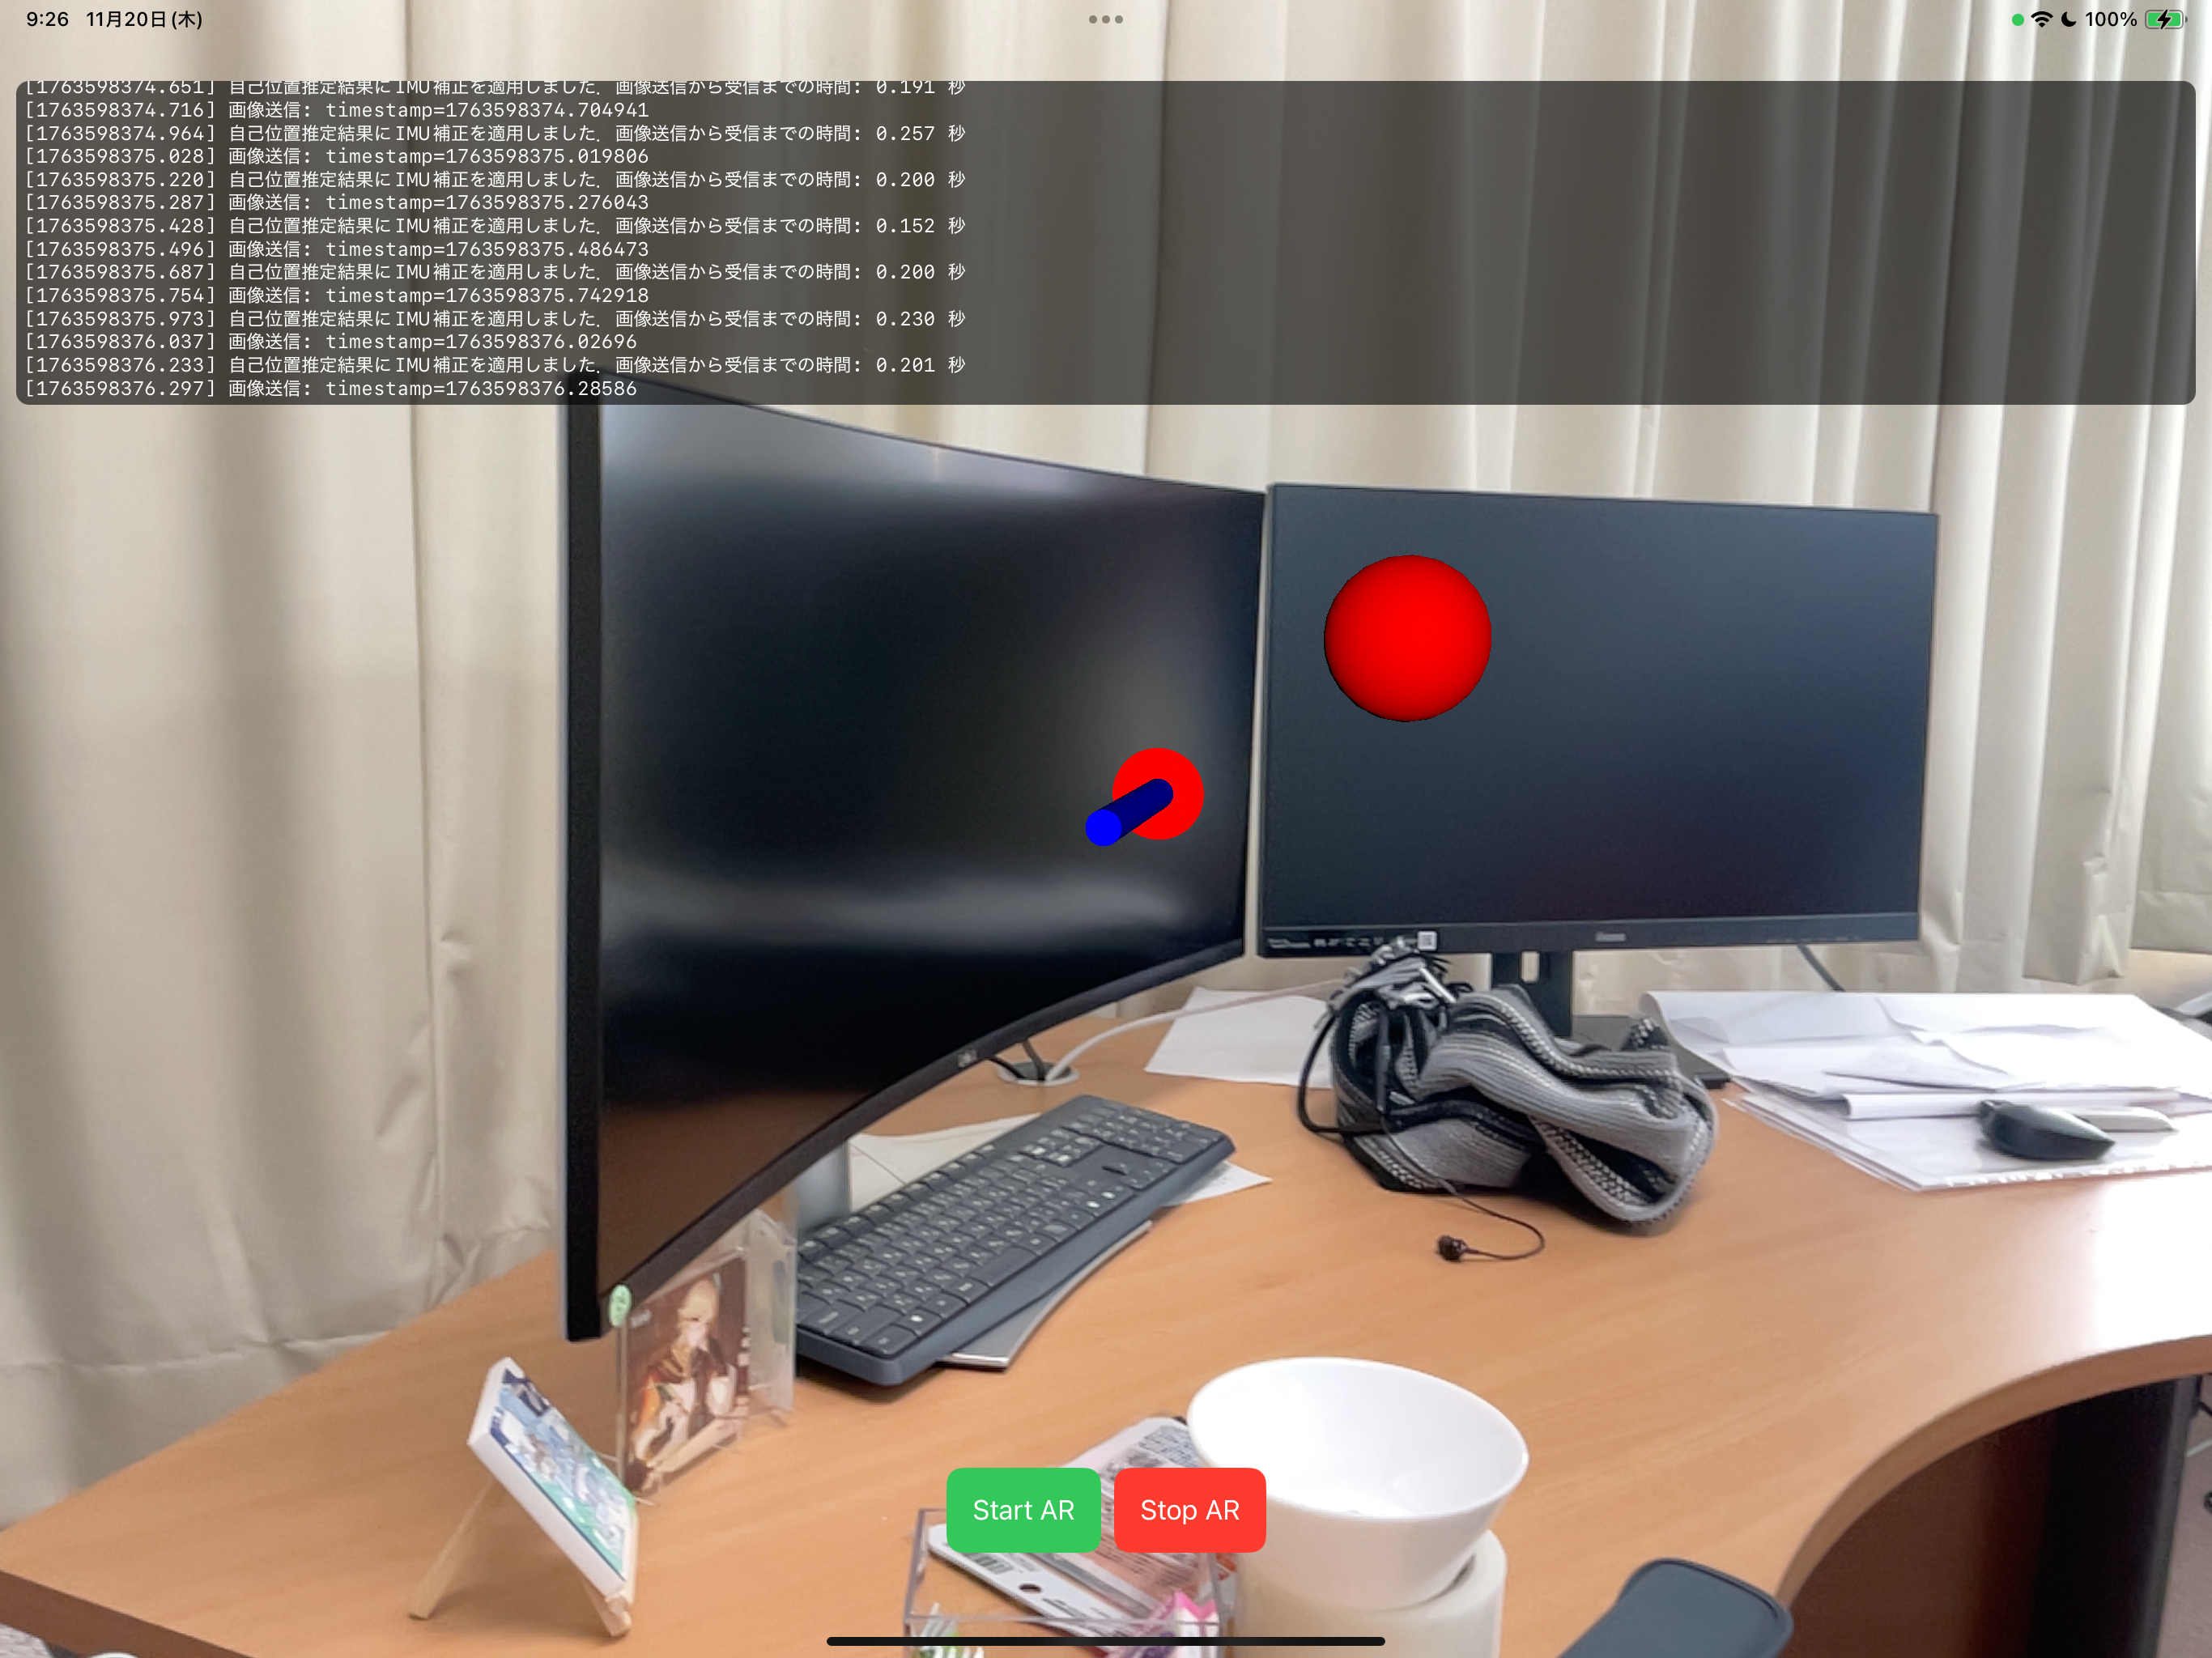
\includegraphics[width=0.4\linewidth]{figures/result_dest1.png} \\
        入力画像 & 目的地1に対する描画結果
    \end{tabular}
    \caption{目的地1に対するオブジェクト描画結果}
    \label{fig:result-dest1}
\end{figure}

\begin{figure}[H]
    \centering
    \begin{tabular}{cc}
        \includegraphics[width=0.4\linewidth]{figures/input_image2.png} &
        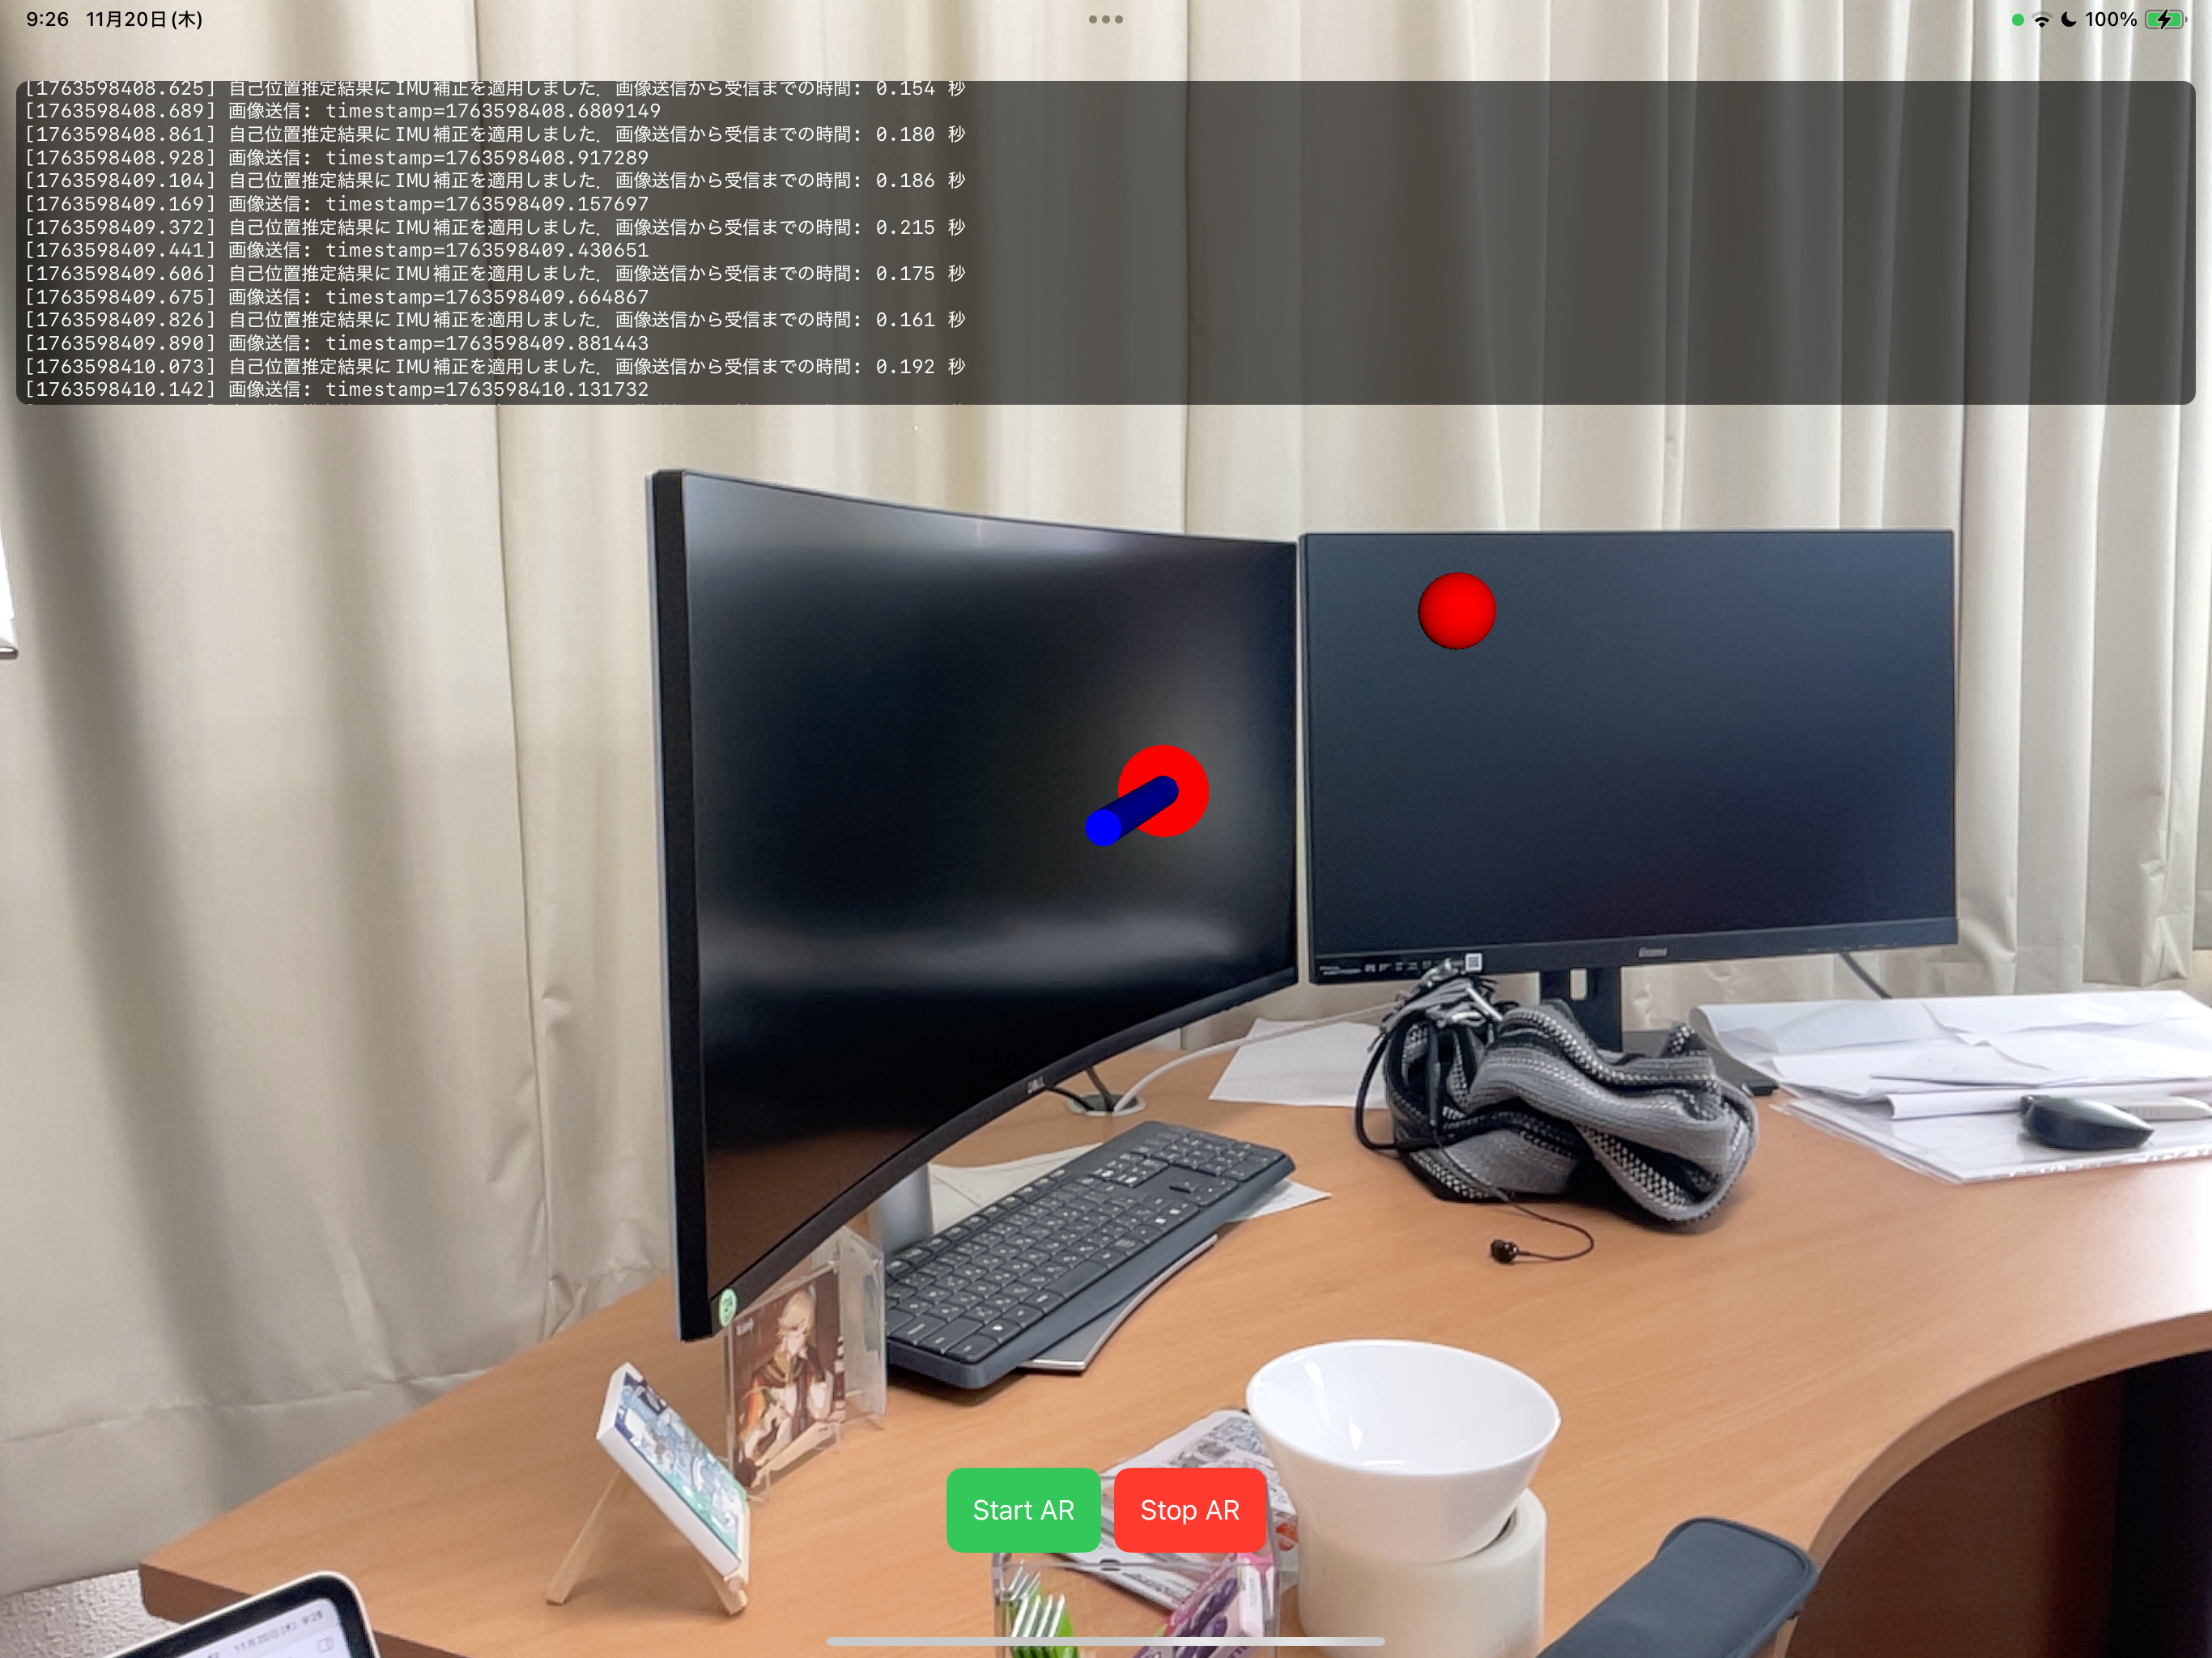
\includegraphics[width=0.4\linewidth]{figures/result_dest2.png} \\
        入力画像 & 目的地2に対する描画結果
    \end{tabular}
    \caption{目的地2に対するオブジェクト描画結果}
    \label{fig:result-dest2}
\end{figure}

より遠い場所を目的地として設定した方が、オブジェクトは小さく描画されていることがわかり、
指定した任意の目的地に対して、対応するオブジェクトはある程度正しく位置に描画されていることを確認した。
また、実行時の動画を
(\href{https://drive.google.com/file/d/11ouiGpY2B3j3JziUIqTNaBzeEzSpID_H/view?usp=drive_link}{result\_1120.mp4})
に示す。

\bibliographystyle{ieeetr}  % または plain, unsrt, apalike などスタイルに応じて選択
\bibliography{reference}   % reference.bib というファイル名を使っている場合

\end{document}
